% Chapter 5

\chapter{Evaluation of the Model} % Main chapter title

\label{Chapter5} % For referencing the chapter elsewhere, use \ref{Chapter5}

% This is for the header on each page - perhaps a shortened title
\lhead{Chapter 5. \emph{Evaluation of the Model}}

% Quotation
``Science, my boy, is made up of mistakes, but they are mistakes which it is useful to make,because
they lead little by little to the truth"

\begin{flushright}
Jules Verne, \textit{Journey to the Centre of the Earth} (1864)
\end{flushright}

%---------------------------------------------------------------------------------------------------
%	CONTENT
%---------------------------------------------------------------------------------------------------

\section{Experimental setup}

We chose a subset of the obtained traffic data for experimentation as shown in the figure
\ref{fig:ExperimentRegion}. The region boundary is denoted by the red line.

\begin{figure}[htbp]
  \centering
    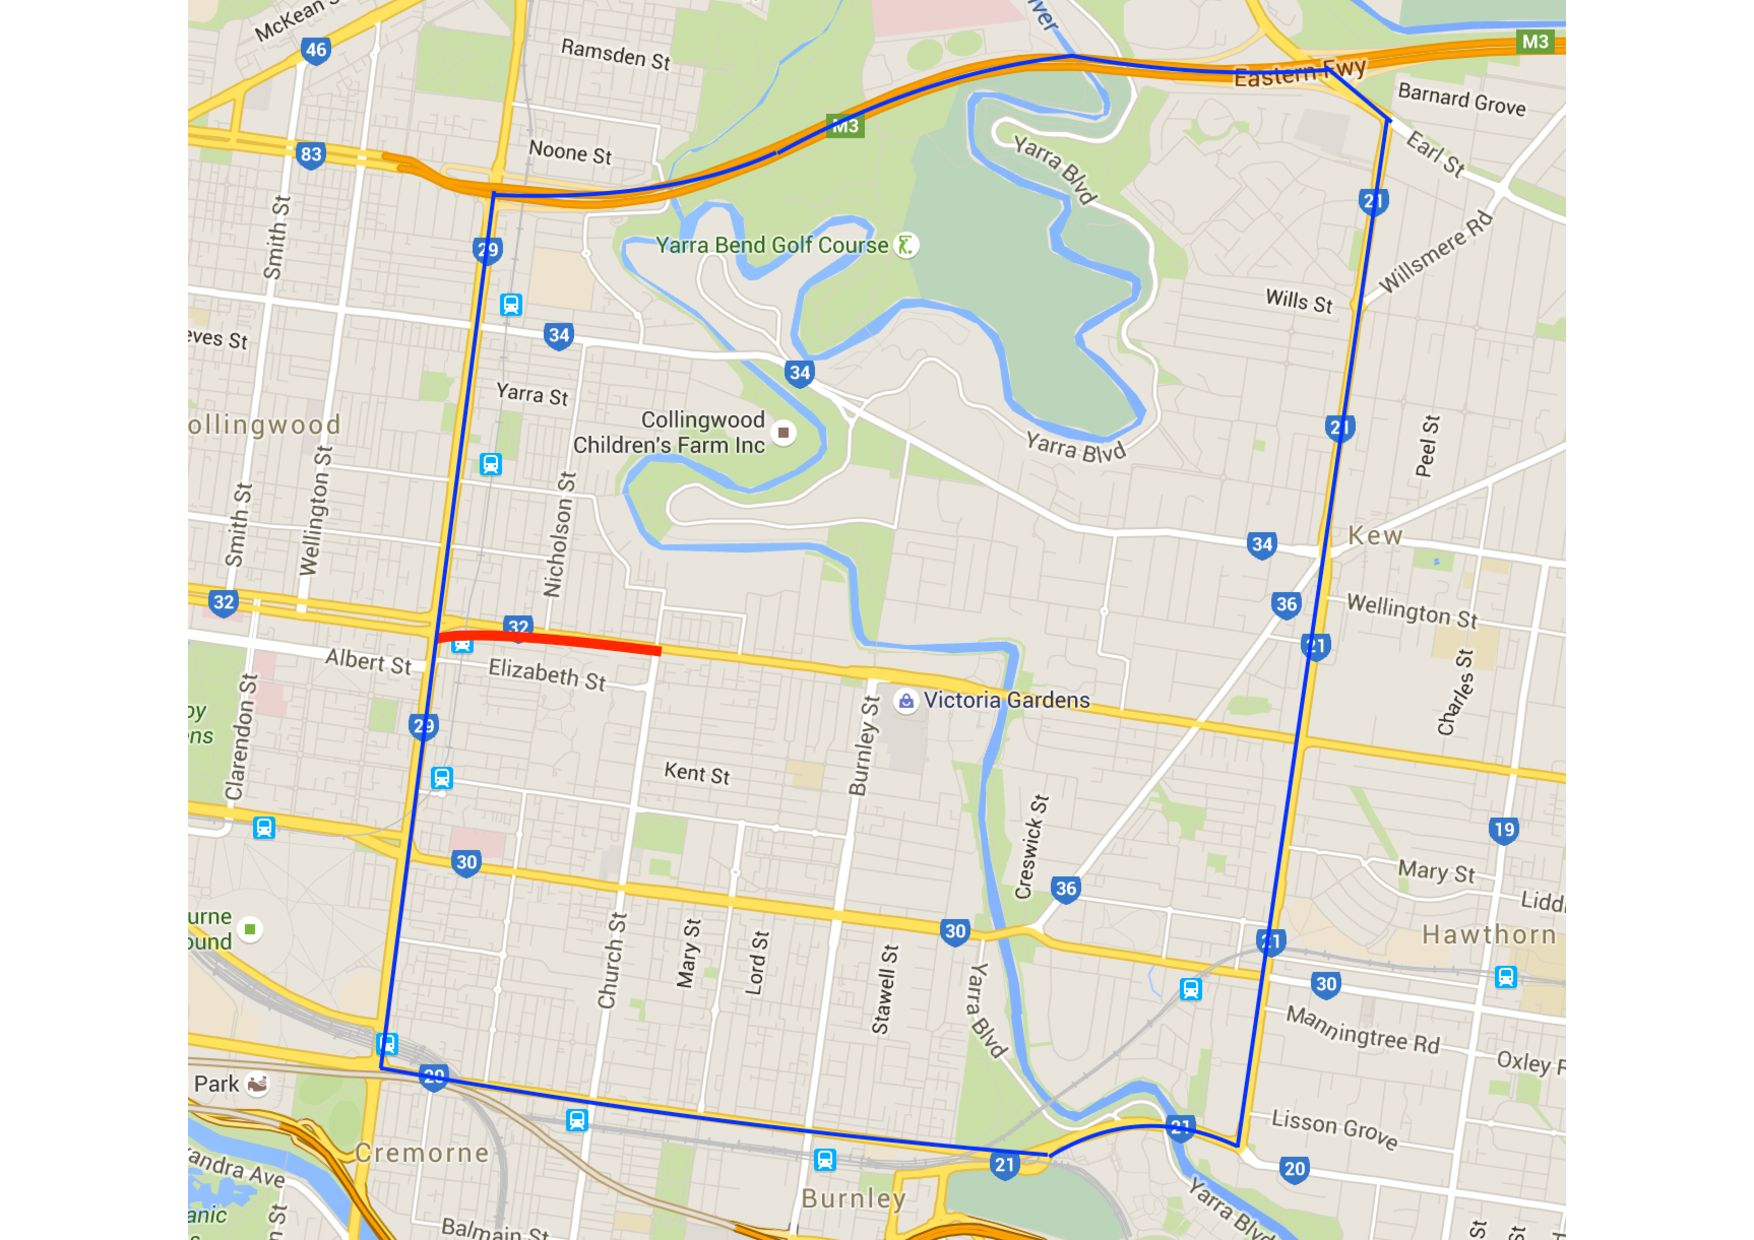
\includegraphics[width=\textwidth,height=\textheight,keepaspectratio]{Figures/experiment-region.pdf}
    \rule{35em}{0.5pt}
  \caption[Experiment traffic region]{The traffic region used in this experiment. The boundary is
   dentoed by the red line.}
  \label{fig:ExperimentRegion}
\end{figure}

\subsection{Training details}


\section{Results}

\begin{figure}[h]
    \centering

    \subfloat[Linear Regression][Linear Regression]{
    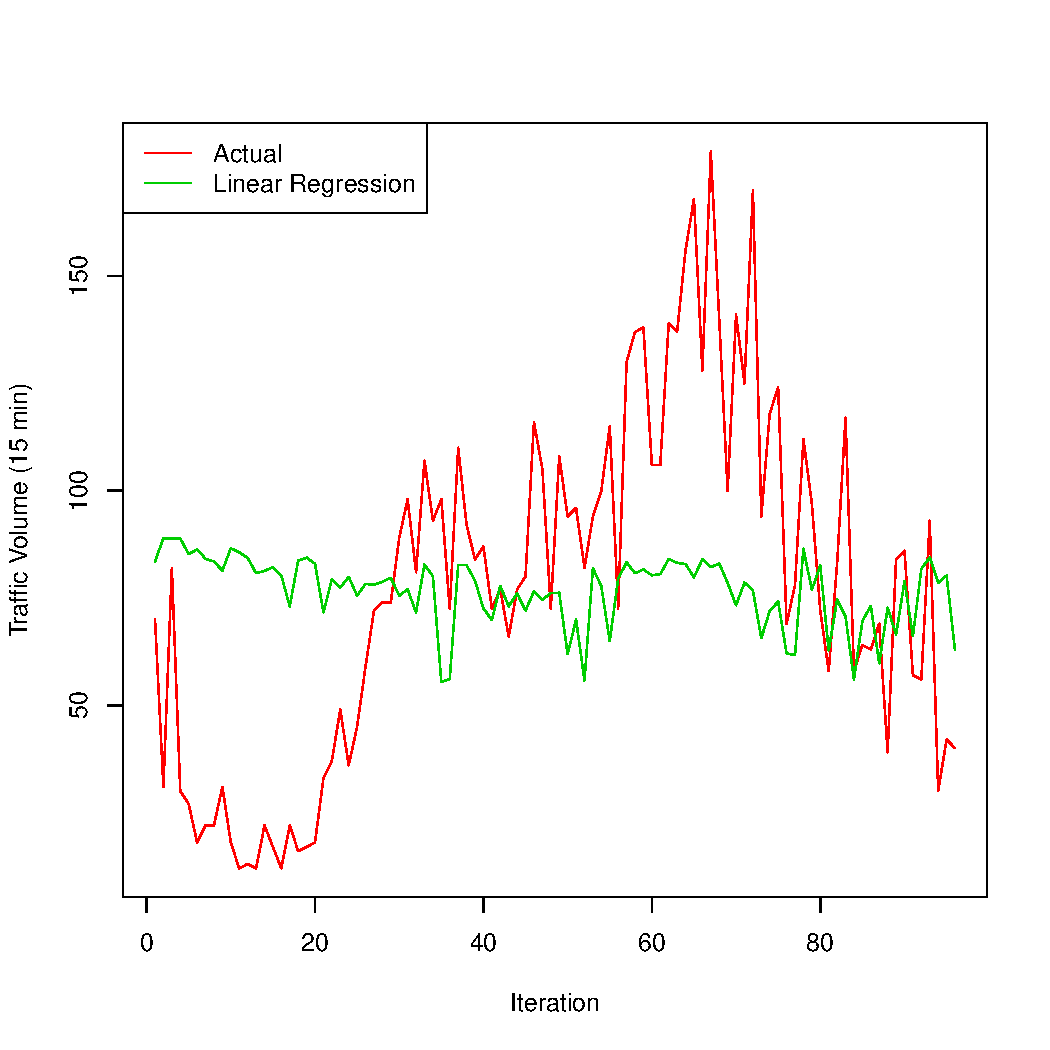
\includegraphics[width=0.4\textwidth]{Figures/linear-regression.pdf}
    \label{fig:LmActualPredicted}}
    \qquad
    \subfloat[ARIMA][ARIMA]{
    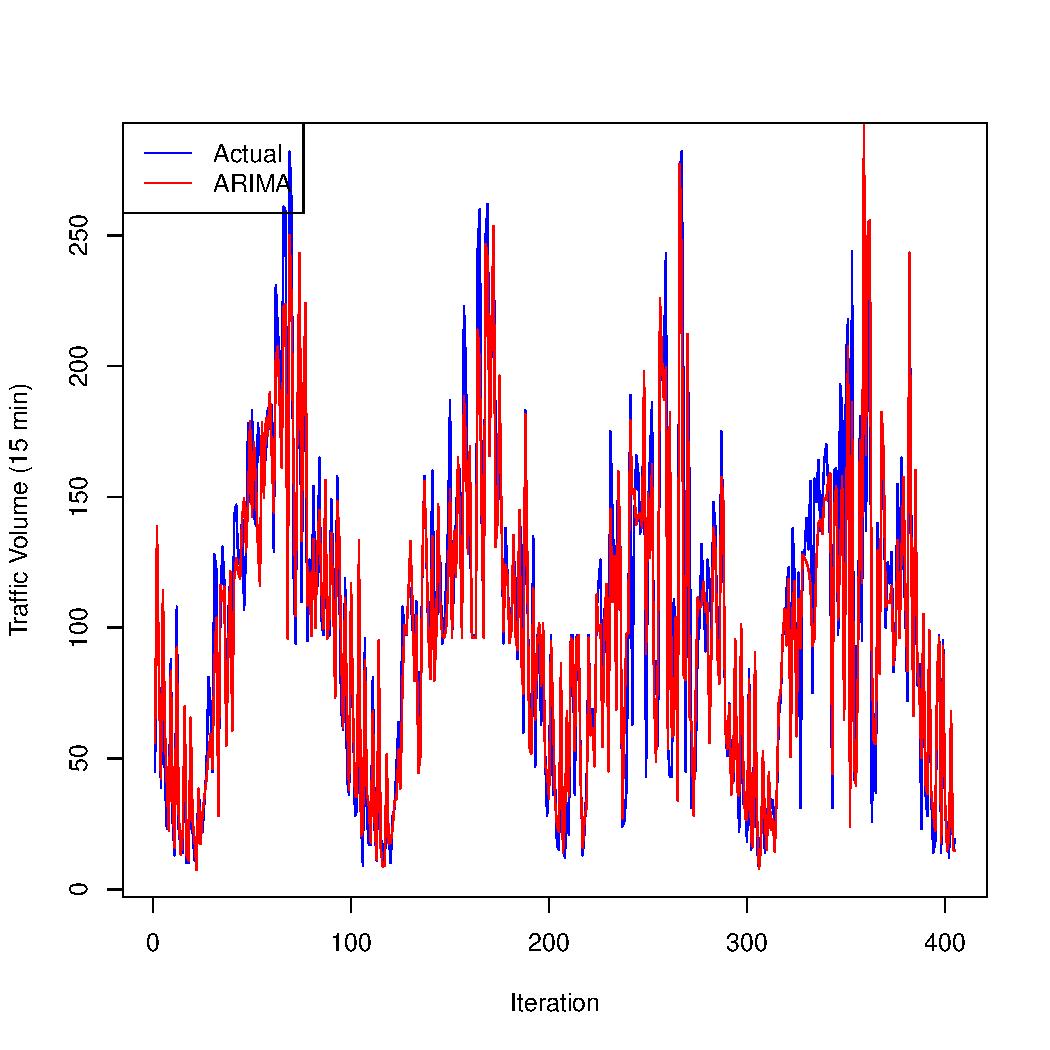
\includegraphics[width=0.4\textwidth]{Figures/arima.pdf}
    \label{fig:ArimaActualPredicted}}

    \subfloat[Exponential smoothing state space model][Exponential smoothing state space model]{
    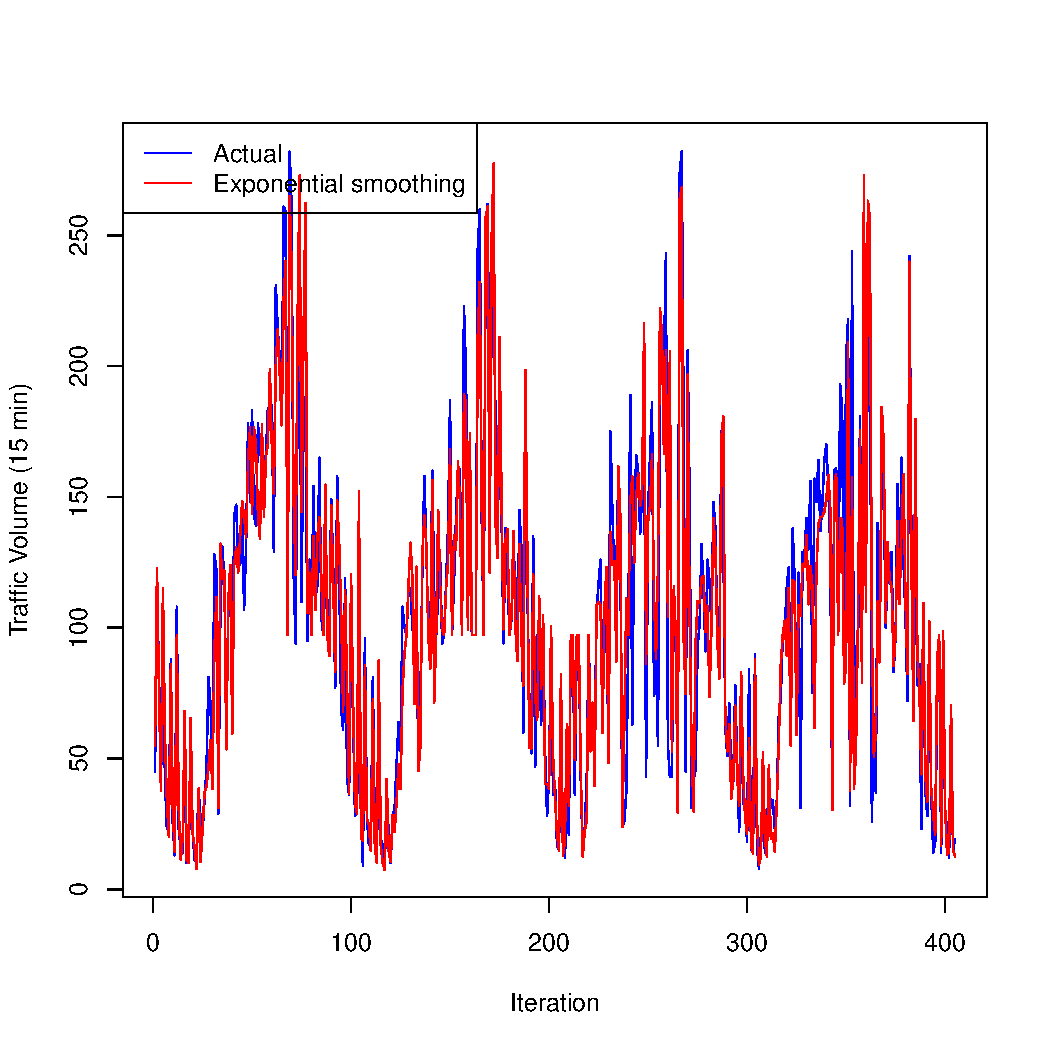
\includegraphics[width=0.4\textwidth]{Figures/exp-smoothing.pdf}
    \label{fig:etsActualPredicted}}
    \qquad
    \subfloat[BP Neural Network][BP Neural Network for time series]{
    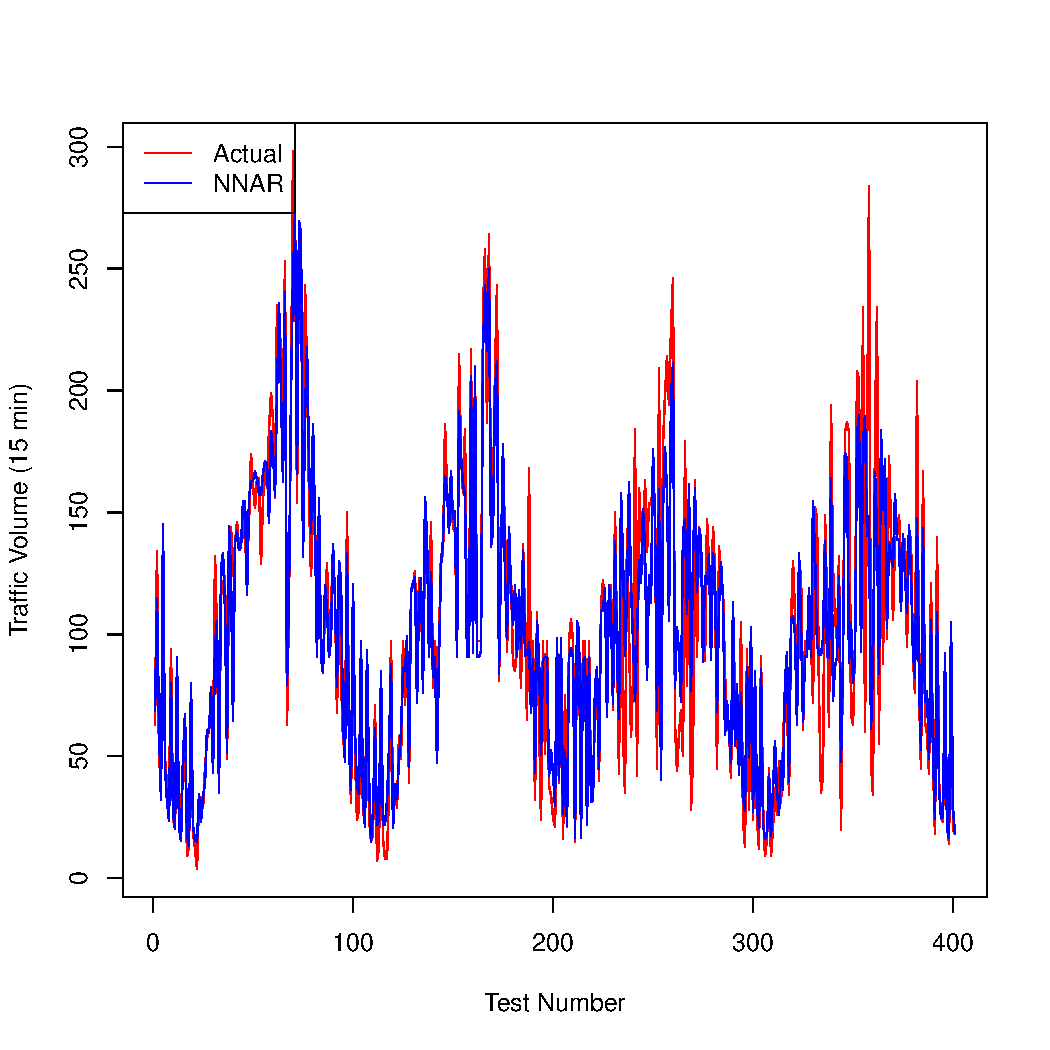
\includegraphics[width=0.4\textwidth]{Figures/nnetar.pdf}
    \label{fig:NnetarActualPredicted}}

    \subfloat[Stacked AutoEncoders][Stacked AutoEncoders]{
    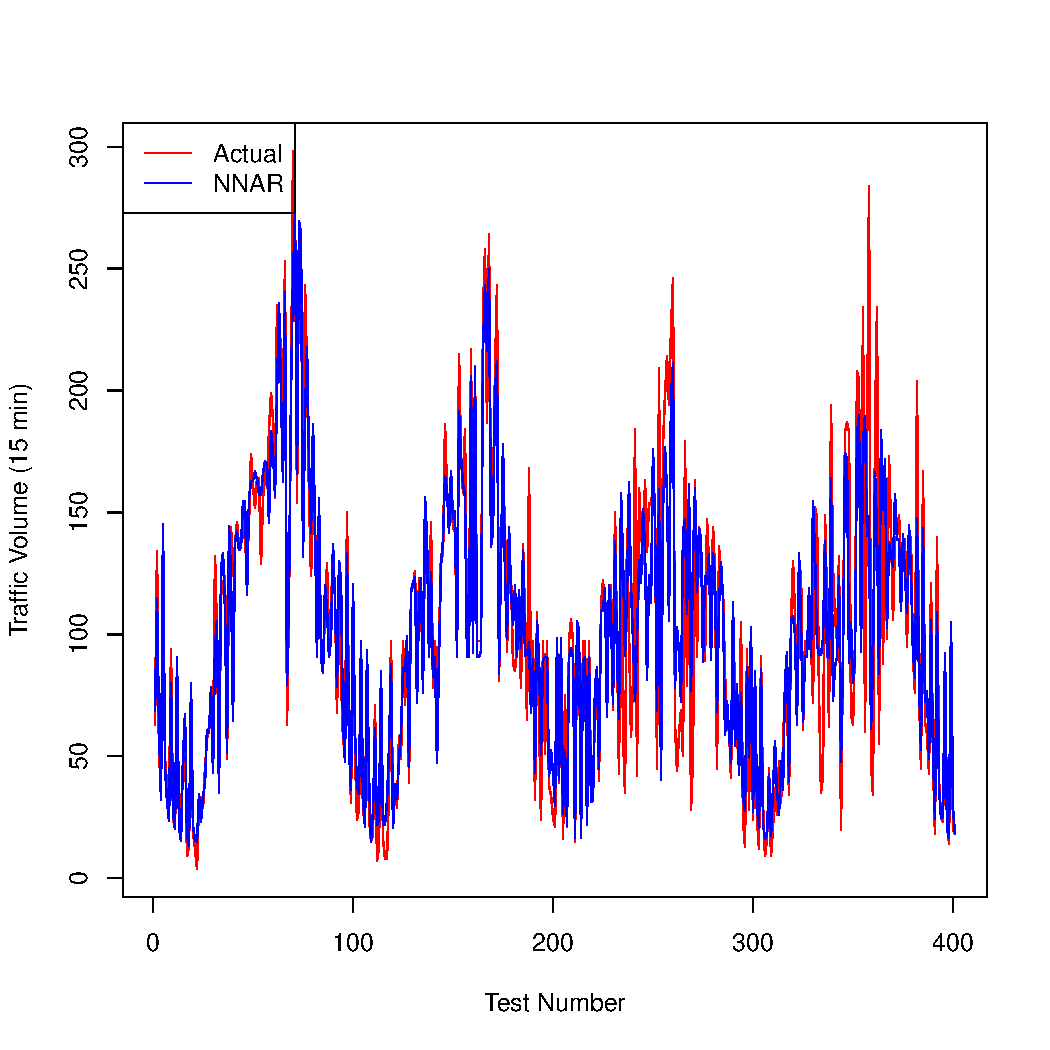
\includegraphics[width=0.4\textwidth]{Figures/nnetar.pdf}
    \label{fig:AutoEncodersActualPredicted}}
    \qquad
    \subfloat[Stacked LSTM][Stacked LSTM]{
    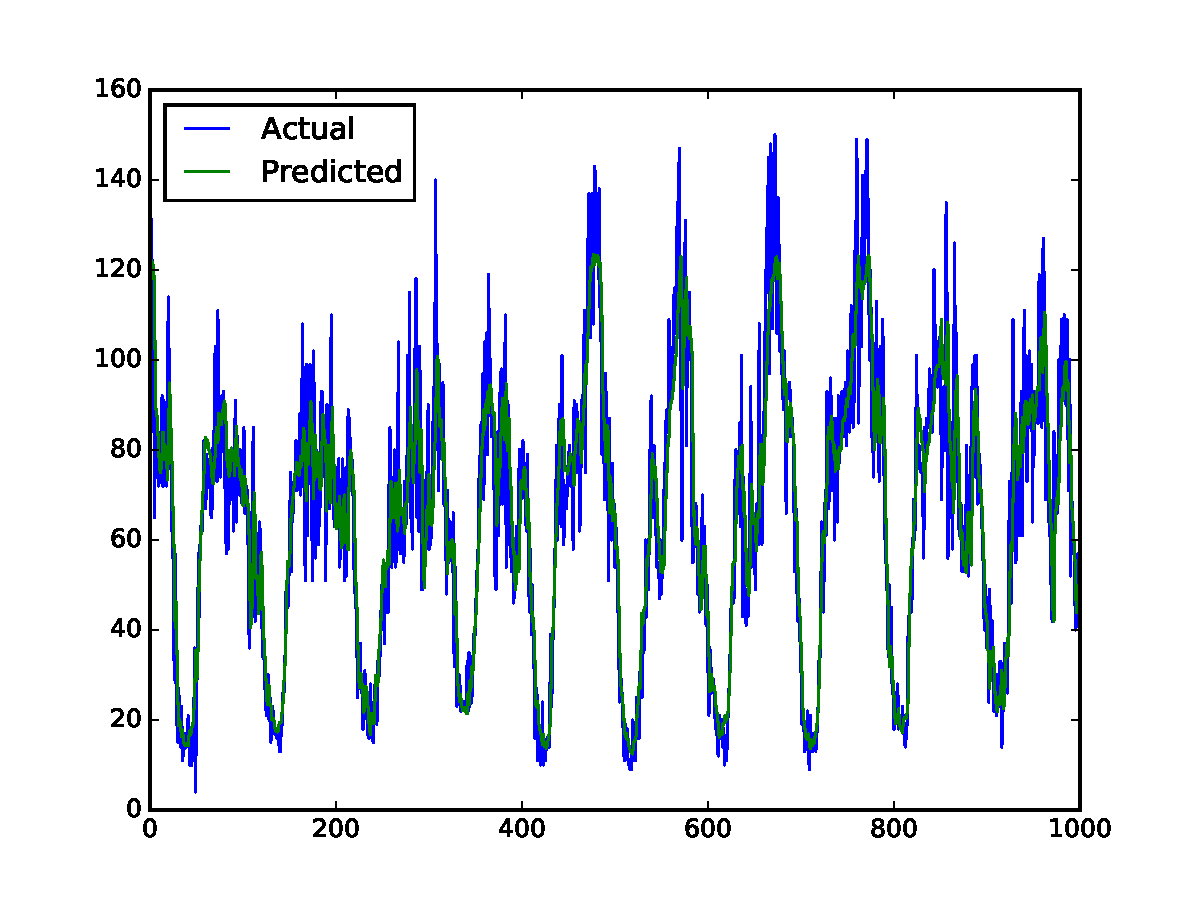
\includegraphics[width=0.4\textwidth]{Figures/lstm.pdf}
    \label{fig:LSTMActualPredicted}}

    \caption[Acutual vs Predictions]{Acutual vs Predictions - Linear regression, ARIMA, BP
    Neural network time series with one hidden layer, Exponential smoothing state space model,
    Stacked Autoencoders and Stacked LSTM network}
    \label{fig:benchmarkModels}
\end{figure}

\section{Evaluation}

Several accuracy measures exist to evaluate a model. In below secions we describe the accuracy
mesures and use those to evalute our proposed model against the benchmark models. For defining
the accuracy measures let us denote $x_{i}$ be the $i^{th}$ observation and $\hat{x}_{i}$ be the
prediction of $x_{i}$.

\subsection{Scale-dependent errors}
The prediction error is simply given by $e_{i} = x_{i} - \hat{x}_{i}$, which is in the same scale
as of the original data. So accuracy measures that depend on $e_{i}$ are scale dependent and can
not be used across multiple series on different scales. The two most used scale-dependent
accuracy measures are mean absolute error and root mean squared error defined as below

    \begin{equation}
        MAE = mean(\abs{e_{i}})
    \end{equation}
    \begin{equation}
        RMSE = \sqrt{mean(e^{2}_{i})}
    \end{equation}

MAE is easy to understand and popular in usage when using a single dataset.

\subsection{Percentage errors}
Percentage errors are scale-independent and thus used across multiple datasets on different
scales. The percentage error is given by $p_{i} = 100*e_{i}/x_{i}$. The most commonly used
percentage measure is Mean Absolute Percentage Error(MAPE) which is given by the below formula
    \begin{equation}
        MAPE = mean(\abs{p_{i}})
    \end{equation}

There are however few shortccomings of the MAPE, for instance when $x_{i}$ is 0 or very large.
Another shortcoming is that they put heavier penalty on negative error values than positve error
values.

\subsection{Scaled errors}
\citet{hyndman2006another} proposed scaled errors to be used as an alternative in place of
percentage errors. The proposed Mean Absolute Scaled Error(MASE) is defined as

    \begin{equation}
        MASE = mean(\abs{q_{i}})
    \end{equation}

where
    \begin{equation}
        q_{i} = \frac{e_{i}}{\frac{1}{T-1} \displaystyle\sum_{t=2}^{T}\abs{x_{t} - x_{t-1}}}
    \end{equation}

A scaled error is less than one if it is better than the average naïve forecast computed on the
training data and vice versa.

\begin{table}
\centering
    \begin{tabular}{| l | l | l| l | l | l | l|} \hline
        Model & \multicolumn{2}{|c|}{RMSE} & \multicolumn{2}{|c|}{MAPE} &\multicolumn{2}{|c|}{MASE} \\
         & 15 mins & 30 mins & 15 mins & 30 mins & 15 mins & 30 mins \\ \hline
        Linear Regression & 201.31 &  & 196.20 &  & 3.31 &  \\
        ARIMA & 41.31 &  & 21.5 &   & 0.64 &  \\
        Eponential Smoothing & 38.97 &   & 14.28 &  & 0.59 &  \\
        BP Neural Network & 51.89 &  & 30.77 &  & 0.87 &  \\
        Stacked Autoencoders &  &  &  &  &  &  \\
        Stacked LSTM &  &  &  &  &  &  \\ \hline
    \end{tabular}
    \caption[Model comparisons]{Accuracy measures - RMSE, MAPE and MASE scores for the evaluted
    models. The scores are calculated for prediction horizon of 15 and 30 minutes}
\end{table}